\begin{wrapfigure}[8]{r}{0.48\textwidth}
     \vspace{-5mm}
  \begin{center}
     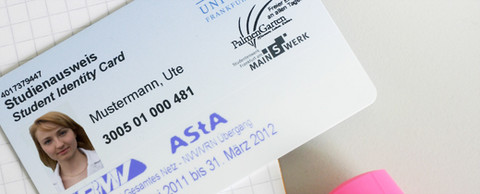
\includegraphics[scale=0.5]{bilder/goethecard}
  \end{center}
\end{wrapfigure}

Nach der erfolgreichen Immatrikulation an unserer Universität bekommst du im Studien-Service-Center eine schicke Chipkarte mit deinem Foto und einigen bildhaften Logos und Beschriftungen drauf. Möglicherweise erfährst du auch gleich, dass sie \emph{Goethe-Card} heißt und als Studienausweis dient. Warum braucht man überhaupt so etwas, wenn man bereits einen ordinären Ausweis hat?

Der wichtigste Grund ist die Tatsache, dass man damit sofort feststellen kann, ob du zum aktuellen Zeitpunkt an der Goethe-Universität studierst: In diesem Fall wurde das blau aufgetragene Gültigkeitsdatum unten zu diesem Zeitpunkt noch nicht überschritten. 

Falls du jetzt ein Blick auf deinen Studienausweis wirfst, wirst du bemerken, dass dort als Enddatum der letzte Tag des laufenden Semesters steht. Daher wirst du, solange du bei uns bleibst, einmal alle 6 Monate diesen Eintrag updaten müssen. Das geht über einen der mehreren extra dafür erstellten und überall auf dem Uni-Gebiet platzierten Automaten, die oft auch \emph{Validierer} genannt werden. Sollte man sein Studium absolviert oder abgebrochen haben, wird der Validierer das Enddatum der Gültigkeit nicht ändern.

Auf der Goethe-Card sind außerdem dein Foto, dein Name und auch deine persönliche Identifikationsnummer (\emph{Matrikelnummer}) in der Universität aufgeschrieben\footnote{Deine Matrikelnummer ist 7-stellig und entspricht den letzten 7 Ziffern der 12\hbox{-}stelligen Zahl auf dem Goethe-Card.}. Diese Angaben helfen nicht nur den Profs, dich eindeutig zu identifizieren, sondern auch dir, deine während der Prüfung vergessene Matrikelnummer schnell zu finden.

Aber das ist noch nicht alles, was du mit der Goethe-Card machen kannst:

\begin{itemize}
	\item Du kannst darauf mittels spezieller Geldautomaten-ähnlichen Geräten darauf \textbf{Geld aufladen}, um damit in der Mensa für das Essen oder auch in der Uni-Bibliothek für die Verwendung des Kopierers zu bezahlen
	\item Du kannst sie als einen \textbf{digitalen Schlüssel} für die super modernen Schließfächer am Campus Westend verwenden
	\item Du kannst damit \textbf{kostenlos} den \textbf{Palmengarten} besuchen
	\item Du kannst damit\textbf{ Bücher in der Uni-Bibliothek ausleihen}
\end{itemize}

Und - last but not least - du kannst damit \textbf{kostenlos} in allen öffentlichen Verkehrsmitteln außer ICE, IC und EC in Hessen fahren! Vor dem 01.03.2013 war das NVV-Gebiet leider nicht mit dabei, daher solltest du deine Goethe-Card unbedingt updaten, wenn du diese vor diesem Tag erhalten hast und kein Logo von NVV neben dem Logo von RMV siehst.

Allerdings pass auf: Außerhalb von Hessen funktioniert das nicht mehr! Auf der nächsten Seite findest du eine Karte mit dem skizzierten Geltungsbereich des Semestertickets.

Ausserdem: Der Verlust der Goethe-Card kann recht schmerzlich sein - z.Z. liegt die Gebühr bei Verlust und darauf folgende Neubeantragung (Campus Westend) bei 50 Euro.

Weitere Informationen zur Goethe-Card kannst du bei Interesse hier finden:\\
\url{http://www.rz.uni-frankfurt.de/44160530/Goethe-Card}
\begin{flushright}Pavel, korrigiert von Sabrina \end{flushright}